\documentclass[bachelor, och, referat, times]{SCWorks}
\usepackage[T2A]{fontenc}
\usepackage[utf8]{inputenc}
\usepackage{graphicx}
\usepackage[sort,compress]{cite}
\usepackage{amsmath}
\usepackage{amssymb}
\usepackage{amsthm}
\usepackage{fancyvrb}
\usepackage{longtable}
\usepackage{array}
\usepackage{multirow}

\usepackage[english,russian]{babel}
\usepackage[colorlinks=true]{hyperref}
\begin{document}


\chair{Дискретной математики и информационных 
технологий}

\title{Семейство операционных систем Linux}

\course{1}

\group{121}

\napravlenie{09.03.01 "--- Информатика и 
вычислительная техника}

\author{Давиденко Алексея Алексеевича}

\chtitle{к. ф.-м.н., доцент}
\chname{Л.Б. Тяпаев}


\satitle{к. ф.-м.н., доцент}
\saname{В.А. Поздняков} 


% Год выполнения отчета
\date{2018}  % в формате ГГГГ

\maketitle

\tableofcontents


\intro Linux - название ядра операционной системы, 
несмотря на то, что это
ядро имеет монолитную архитектуру и не считается 
прогрессивным, оно
поддерживает большинство современных технологий, 
является
многопользовательским и многозадачным. Эта 
операционная система является
третьей по популярности на сегодняшний день. Она 
установлена на огромном
количестве компьютеров и составляет достойную 
конкуренцию операционным
системам разрабатываемым гигантскими корпорациями, 
несмотря на то, что
разрабатывается, в основном, добровольцами-
энтузиастами.

\section{ИСТОКИ LINUX}

\par Справедливо считается, что Linux имеет двух 
$\textrm {прародителей}\raisebox{1ex}{\scriptsize ~рис.~\ref{fig:hist}}$, на 
основании которых он и возник. 
Это операционная система $\textrm{UNIX}
\raisebox{1ex}{\scriptsize ~рис.~\ref{fig:UNIX_symbol}}$ и проект 
$\textrm{GNU}\raisebox{1ex}{\scriptsize ~рис.~\ref{fig:GNU_symbol}}$. О них будет 
рассказано ниже.

\par Linux является {Unix-подобной}\footnote{Unix-подобная операционная система — операционная система, которая образовалась под влиянием Unix.} операционной 
системой, совместимой с 
ней. Первая система Unix была разработана в 1969г. 
в подразделении Bell 
Labs компании AT\&T. В те времена компании AT\&T 
было запрещено заниматься
компьютерным бизнесом, поэтому операционная система 
Unix распространялась 
бесплатно и её исходные коды были открыты. Это 
обстоятельство 
способствовало распространению системы в 
университетской среде, и 
стремительному её развитию. Студенты и профессора 
вносили в неё улучшения,
создавали для неё утилиты. Коммерческие компании 
разрабатывали клоны 
системы Unix. Система стремительно набирала 
популярность и была 
установлена на множестве компьютеров. В 1983 году 
был реализован стек 
протоколов TCP/IP, что значительно расширило её 
сетевые возможности. В 
итоге, в 80-х годах, накал борьбы между 
производителями Unix-ов достиг 
максимума. В 1983 с корпорации AT\&T был снят 
запрет на занятие 
компьютерным бизнесом. Она занялась 
коммерциализацией свой разработки. 
Были закрыты исходные коды системы, а компании 
использующие эти коды, 
подвергались патентным преследованиям. После 
нескольких лет таких 
UNIX-войн развитие Unix практически сошло на нет. И 
UNIX уступила место на
компьютерах конкурирующим системам, в частности MS 
DOS и Apple Macintosh.

\par Вторым прародителем Linux, можно считать 
проект GNU 
\href{https://en.wikipedia.org/wiki/Richard_Stallman}{Ричарда 
Столлмана}. Он возник в 1983 году, и его целью было 
создание полностью 
свободной операционной системы. Толчком к рождению 
проекта стали 
обстоятельства возникшие в 1982 году. Тогда Ричард 
Столлман работал в 
лаборатории искусственного интеллекта 
Массачусетского Технологического 
Института. В их лабораторию была куплена 
коммерческая операционная 
система. Условия лицензирования этой системы 
накладывали ограничения на 
распространение исходных кодов программ, и это 
заметно тормозило процесс 
разработки программного обеспечения, требовало 
повторной разработки уже 
существующих компонентов. Ричард Столлман, сам 
будучи очень талантливым 
программистом решил переломить это порочное 
положение вещей в 
программировании. 27 сентября 1983 года он объявил 
о начале разработки 
проекта GNU (GNU is Not Unix) целью которого было 
создание 
Unix-совместимой операционной системы, у которой 
будет ядро и все 
необходимые сопутствующие утилиты (редактор, 
оболочка, компилятор и т.д.).
Так же декларировалась возможность получения 
исходных кодов проекта любым 
желающим. Все желающие приглашались к участию в 
проекте. Чтобы МТИ не мог 
навязать права собственности на детище Столлмана, 
он ушел из института в 
январе 1984. Первой программой, разработанной в 
рамках проекта был 
текстовый редактор Emacs. В 1985 году Столлман 
основал Free Software 
Foundation (FSF) - благотворительный фонд для 
разработки свободно 
распространяемого ПО. Следующим очень важным шагом 
Ричарда было создание 
лицензии GPL (General Public License). Основная 
идея GPL в том, что 
пользователь должен обладать следующим правами 
(свободами):
	\begin{enumerate}
		\item Правом запускать программу для любых 
		целей;
		\item Правом изучать устройство программы и 
		приспосабливать ее к 
		своим потребностям, что предполагает доступ 
		к исходному коду 
		программы;
		\item Правом распространять программу, имея 
		возможность помочь 
		другим;
		\item Правом улучшать программу и 
		публиковать улучшения, в пользу 
		всего сообщества, что тоже предполагает 
		доступ к исходному коду 
		программы.
	\end{enumerate}
	
\par Программное обеспечение, распространяемое под 
этой лицензией, можно 
как угодно использовать, копировать, дорабатывать, 
модифицировать, 
передавать, продавать модифицированные (или 
немодифицированные) версии 
другим лицам при условии, что результат такой 
переработки тоже будет 
распространяться под лицензией GPL. Последнее 
условие - самое важное и 
определяющее в этой лицензии. Оно гарантирует, что 
результаты усилий 
разработчиков свободного ПО останутся открытыми и 
не станут частью 
какого-либо проприетарного продукта.

\par К 1990 году в рамках проекта GNU было создано 
большинство компонент, 
необходимых для функционирования свободной 
операционной системы. Помимо 
текстового редактора Emacs, Столлман создал 
компилятор gcc (GNU C 
Compiler) и отладчик gdb. Так-же были разработаны 
библиотека языка Си и 
оболочка BASH. Недоставало только самого важного - 
ядра. В это самое время
и появилась на свет разработка финского студента 
Линуса Торвальдса - ядро 
Linux. Можно сказать, что появилось оно в нужное 
время. И теперь симбиоз 
этих двух разработок зовется GNU/Linux.

\section{РОЖДЕНИЕ LINUX}

\par \href{https://en.wikipedia.org/wiki/Linus_Torvalds}{Линус Бенедикт Торвальдс} родился 28 
декабря 1969 года. В школе
он был отличным математиком, и ещё с детства начал 
увлекаться 
компьютерами. После окончания школы, он поступил в 
Университет Хельсинки 
на отделение компьютерных наук. Тогда у него был 
персональный компьютер на
основе процессора Intel 80386 с 4 мегабайтами ОЗУ и 
тактовой частотой 33 
мегагерца. Под впечатлением от книги Эндрю С. 
Таненбаума (разработчика 
учебной операционной системы Minix)~"Проектирование 
и реализация 
операционных систем"\,, Линус установил на свой 
компьютер ОС 
$\textrm{Minix}\raisebox{1ex}{\scriptsize ~рис.~\ref{fig:minix_symbol}}
$. Однако, молодого студента далеко 
не всё устраивало в этой системе. Больше всего 
нареканий вызывала работа 
терминала с помощью которого он подключался к 
компьютеру университета, а 
через него и к глобальной сети интернет. Линус 
принялся писать собственный
терминал. После того как терминал был готов, 
возникала проблема со 
скачиванием и загрузкой файлов. Пришлось писать 
драйвера для 
флоппи-дисковода, а следом и собственную файловую 
систему, так как у
файловой системы Minix были проблемы с 
многозадачностью. Так из попытки 
написания терминала появился скелет будущей 
операционной системы. Линуса 
заинтересовала идея создания собственной ОС и он 
принялся за разработку. 
25 августа 1991 года Торвальдс написал e-mail в 
список рассылки 
пользователей Minix, в котором сообщал, что 
занимается разработкой 
операционной системы и просил указать пожелания и 
предложения от 
пользователей Minix. Этот день считается днём 
рождения Linux. А 5 октября 
он выпустил версию ядра 0.2 и выложил исходные коды 
в интернет. Многие 
заинтересовались этой системой. У Линуса появились 
помощники, работа 
закипела. 05.01.1992 была выпущена версия 0.12 под 
лицензий GPL, Linux 
стал достоянием всего мира. Версия 0.96 была 
выпущена в апреле 1992, в ней
появилась возможность работы графической подсистемы 
X Window. И только 
через два года, 16.04.1994 вышел первый стабильный 
релиз - версия 1.0. К 
этому времени в рядах разработчиков уже были тысячи 
человек. Система 
динамично развивалась. В ней функционировало 
множество прикладного ПО. 
Промышленные компании и мелкие фирмы начали 
разрабатывать, продавать и 
встраивать в устройства свои версии открытой ОС. 
Зародились дистрибутивы 
Linux.

\par Дистрибутив Linux - это набор пакетов 
программного обеспечения, 
включающий базовые компоненты операционной систем 
(в том числе, ядро 
Linux), некоторую совокупность программных 
приложений и программу 
инсталляции, которая позволяет установить на 
компьютер пользователя 
операционную систему GNU/Linux и набор прикладных 
программ, необходимых 
для конкретного применения системы. Т.е. эта 
законченная, 
полнофункциональная система, уже адаптированная для 
применения конечным 
пользователем, а не только разработчиком.

\par Первые дистрибутивы Linux появились вскоре 
после того, как Линус
Торвальдс выпустил разработанное им ядро под 
лицензией GPL. Отдельные 
программисты (и группы программистов) начали 
разрабатывать как программы 
инсталляции, так и другие прикладные программы, 
пользовательский 
интерфейс, программы управления пакетами и 
выпускать свои дистрибутивы.

\par Первый дистрибутив Linux был создан Оуэном Ле 
Бланк в феврале 1992 
(Англия). В октябре 1992 появился разработанный 
Питером Мак-Дональдом 
дистрибутив Softlanding Linux System, который 
включал в себя такие 
элементы, как X Window System и поддержка TCP/IP. В 
конце 1992 года Патрик
Фолькердинк выпустил дистрибутив который он назвал 
"Slackware" и который 
является старейшим дистрибутивом из тех, которые до 
сих пор активно 
развиваются. На основе дистрибутива Slackware 
германской фирмой S. U. S. 
E, был создан дистрибутив SuSE Linux, версия 1.0 
которого вышла в 1994 
году. Еще один проект по разработке дистрибутива, 
Debian, был начат Яном 
Мёрдоком 16 августа 1993 года как альтернатива 
коммерческим дистрибутивам 
Linux. Дистрибутив Red Hat, был основан в 1994 
году. На основе Red Hat 
было создано множество других дистрибутивов.

\section{РАЗВИТИЕ LINUX}

\par После выпуска версии 1.0, ядро продолжило свое 
развитие в виде двух 
веток - стабильной (рекомендуемой к широкому 
использованию) и 
экспериментальной (тестовая версия, включающее 
новые возможности и активно
разрабатываемое). Стабильные версии имели чётную 
вторую цифру в номере 
(например 1.0.1), а экспериментальные нечётную 
(например 1.1.4). После 
того как экспериментальная версия была достаточно 
обработана и годилась к 
использованию широкими слоями пользователей, её 
второй номер увеличивался 
на единицу и она считалась стабильной. Одновременно 
с этим появилась новая
экспериментальная версия.

\par Разработка Linux всё время набирала обороты. 
Если в версии 0.1 
имелось всего 8 400 строк кода, то в версии 1.0 уже 
170 000. В июне 1996 
система уже поддерживала множество архитектур, и 
многопроцессорную 
технологию. Дальнейшее развитие в основном было 
направленно на улучшение 
производительности, поддержке новых технологий и 
аппаратных средств. 
Вообще, именно на последний пункт, приходилась 
большая часть кода ядра, 
которая к январю 2001 года превышало число в 3 000 
000 строк. Программисты
стремились создавать драйвера для как можно 
большего количества 
оборудования. Порою это было не простой задачей, 
т.к. многие производители
не считали систему заслуживающей внимания, не 
писали для неё драйверов и 
не открывали спецификации на свои устройства.

\par В это время Торвальдс уже практически отошел 
от прямой разработки 
ядра, и его основной обязанностью стало руководство 
процессом разработки. 
Он выбирал направления развития и принимал решения 
о включении патчей, 
присылаемых ему разработчиками со всего мира. Кроме 
того Линус распределял
полномочия по руководству разработкой отдельных 
направлений различным 
участникам сообщества, сам же сосредоточился на 
основополагающих 
компонентах.

\par В 1996 году был выбран символ 
$\textrm{системы}\raisebox{1ex}{\scriptsize ~рис.~
\ref{fig:linux_symbol}}$. Им стал 
добродушный и в меру 
упитанный пингвинёнок Такс, отличительная 
особенность которого - жёлтые 
лапы и клюв.

\par Одной из проблем этого времени стала 
стандартизация. Дистрибутивов 
становилось всё больше, многие из них были похожи 
друг на друга, другие 
разительно отличались по многим параметрам, начиная 
от структуры файловой 
системы и системы инициализации и заканчивая 
используемыми библиотеками и 
конфигурацией ядра. Это обстоятельство имело свои 
негативные последствия. 
Разработчикам приходилось адаптировать свои 
программы под различные 
дистрибутивы, на это уходило много сил и средств. 
Первым проектом по 
стандартизации был Filesystem Standart project 
(FSSTND). Он стартовал в 
августе 1993, и стандартизировал организацию 
файловых систем. Позже был 
переименован в Filesystem Hierarchy Standard или, 
FHS. В мае 1998 года 
стартовал проект Linux Standart Base (LSB), он 
должен был определить набор
тех компонент, которые должны присутствовать в 
любой "Linux-системе". 
Инициаторы проекта ставили цель обеспечить бинарную 
совместимость 
дистрибутивов, удовлетворяющих стандарту LSB. 
Велись и другие проекты по 
стандартизации.

\section{РАСПРОСТРАНЕНИЕ LINUX}
\par Широкое распространение операционной системы 
Linux началось со 
времени выхода стабильной версии ядра версии 2.2 в 
январе 1999 года. На 
нее обратили внимание производители серверных 
приложений, баз данных, 
Web-серверов, а также приложений для всякого рода 
защиты ПК. Произошло это
во многом благодаря широкому распространению веб-
сервера Apache. На 
сегодняшний день порядка 65\% web-серверов работают 
на ОС Linux, по данным
TOP500, Linux используется на 91 \% самых мощных 
суперкомпьютеров планеты 
и на подавляющее большинстве компьютеров 
обслуживающих систему доменных 
имён DNS (без которой не возможно функционирование 
сегодняшней сети 
интернет). Инфраструктура самой популярной 
поисковой системы Google.com и 
сайта wikipedia.org (шестого в мировом рейтинге), 
строится на базе 
множества серверов с Linux. Можно сказать, что на 
серверах Linux чувствует
себя уверенно и пришел на них на долго.

\par Начиная с 1998 года, о поддержке, 
распространении и продаже Linux 
начали заявлять крупнейшие IT-компании - гиганты 
компьютерного рынка. В их
число входят: Sun, IBM, Oracle, Hewlett-Packard, 
Novell. Эти компании 
начали устанавливать Linux на свои сервера, 
адаптировать под него свои 
программные продукты. По-другому взглянули на 
свободное программное 
обеспечение и правительства стран, администрации 
городов. Зачастую они 
стали отказываться от продуктов корпорации 
Microsoft в пользу Linux и СПО,
экономя при этом, огромные деньги. В число таких 
стран входят Германия, 
Франция, Англия, Япония. Порой целые города, 
муниципальные службы и 
министерства в них переходили на СПО.

\par Так же большую популярность, благодаря своей 
гибкости и свободности, 
Linux завоевал на различных встраиваемых и 
мобильных устройствах. Порой мы
даже не подозреваем об обилии Linux вокруг нас. 
Различные модемы и 
роутеры, терминалы и тонкие клиенты, промышленные 
станки и системы 
видеонаблюдения, коммуникаторы и смартфоны. 
Диапазон применения системы 
очень широк.

\par Несколько другая ситуация на рынке настольных 
систем. Там царит 
гегемония продуктов Microsoft. По разным оценкам, 
доля ОС Linux составляет
порядка 1\% -5\% от общего числа. Этому есть целый 
рад причин. Во-первых, 
долгое время в Linux отсутствовали программы к 
которым пользователи 
привыкли в среде Windows. В частности это 
относилось к офисным пакетам, 
программам обработки звука, инженерными системам и 
играм. На данный момент
ситуация гораздо лучше, но всё же не идеальна. 
Вторая причина - поддержка 
аппаратных средств. Далеко не все производители 
выпускают драйвера для ОС 
Linux, ввиду малочисленности их пользователей. 
Драйвера приходится писать 
энтузиастам, зачатую устройства имеют ограниченную 
функциональность, а то 
и вовсе не работают. Хотя и здесь ситуация за 
последнее время значительно 
изменилась в лучшую сторону. Сегодня поддерживается 
огромное количество 
устройств, и каждый день этот список расширяется. К 
тому же многие 
производители периферии осознали значимость Linux, 
и сами стали выпускать 
драйвера для своих продуктов. И последняя причина, 
это банальная привычка.
Для многих Windows и компьютер стали синонимами, и 
освоение новой системы 
их пугает. Усугубляется это тем, что изначально, 
конфигурирование Linux, 
предполагает работу в командной строке, а 
графическая оболочка это лишь 
удобная надстройка для повседневной работы. Многим 
этот принцип кажется 
сложным. Не говоря о гибкости и широких 
возможностях командного 
интерфейса, можно сказать что современные 
дистрибутивы вроде Ubuntu 
предоставляют богатый инструментарий по настройке 
именно в графическом 
интерфейсе. К тому же установка этого дистрибутива 
на компьютер не сложнее
установки Windows, т.к. один из главных принципов 
построения этого 
дистрибутива - дружелюбный для пользователя 
интерфейс.

\par Благодаря изменениям последних лет, число 
инсталляций Linux всё время
растёт. Ясно что эта система имеет большое будущее. 
В компьютерных 
магазинах, зачатую, помимо Windows, можно увидеть 
Linux как 
предустановленную систему. В России идёт процесс 
внедрения Linux и 
свободного программного обеспечения в школах и 
государственных 
учреждениях.

\conclusion

То, что зарождалось как программа для подключения к 
университетскому 
компьютеру, превратилось в самый грандиозный проект 
мира свободного 
программного обеспечения. Сегодня по данным 
Евросоюза, стоимость 
разработки ядра Linux с нуля при коммерческом 
подходе, составляет более 
одного миллиарда евро. Модель коллективной 
разработки СПО доказала свою 
жизнеспособность. Для многих оказалось открытием, 
возможность достойной 
конкуренции разработки кучки энтузиастов против 
продуктов 
транснациональных корпораций с многомиллиардными 
оборотами. Linux в 
очередной раз, доказал, что деньги в этом мире не 
главное, и добрая воля 
человека способна на великие свершения.

\begin{thebibliography}{99}
	\bibitem{Ione} Костромина В.А. "Свободная 
	система для свободных 
	людей", 2005г.,
	\href{http://www.linuxcenter.ru/lib/history/
	lh-00.phtml}{http://www.li
	nuxcenter.ru/lib/history/lh-00.phtml}
	
	\bibitem{Itwo} Федорчук Алексей "Linux: 
	предыстория в тезисах", 
	2006г.,
	\href{http://www.linuxcenter.ru/lib/history/
	linuxhistory_1.phtml}{http
	://www.linuxcenter.ru/lib/history/linuxhistory
	\_1.phtml}
	
	\bibitem{Ithree} Статьи с сайта
	\href{http://ru.wikipedia.org}{http://
	ru.wikipedia.org}
	
	\bibitem{Ifour} Далхаймер М., Уэлш М. 
	"Запускаем Linux", 2008г., 
	Символ-Плюс.
	
	\bibitem{Ifive} Маянк Шарма. Рождение ядра 
	Linux, 2016г., — Октябрь (№
	10 (215)). — С. 24-31.
\end{thebibliography}

\appendix

\section{Изображения}

\begin{figure}[h]
    \centering
    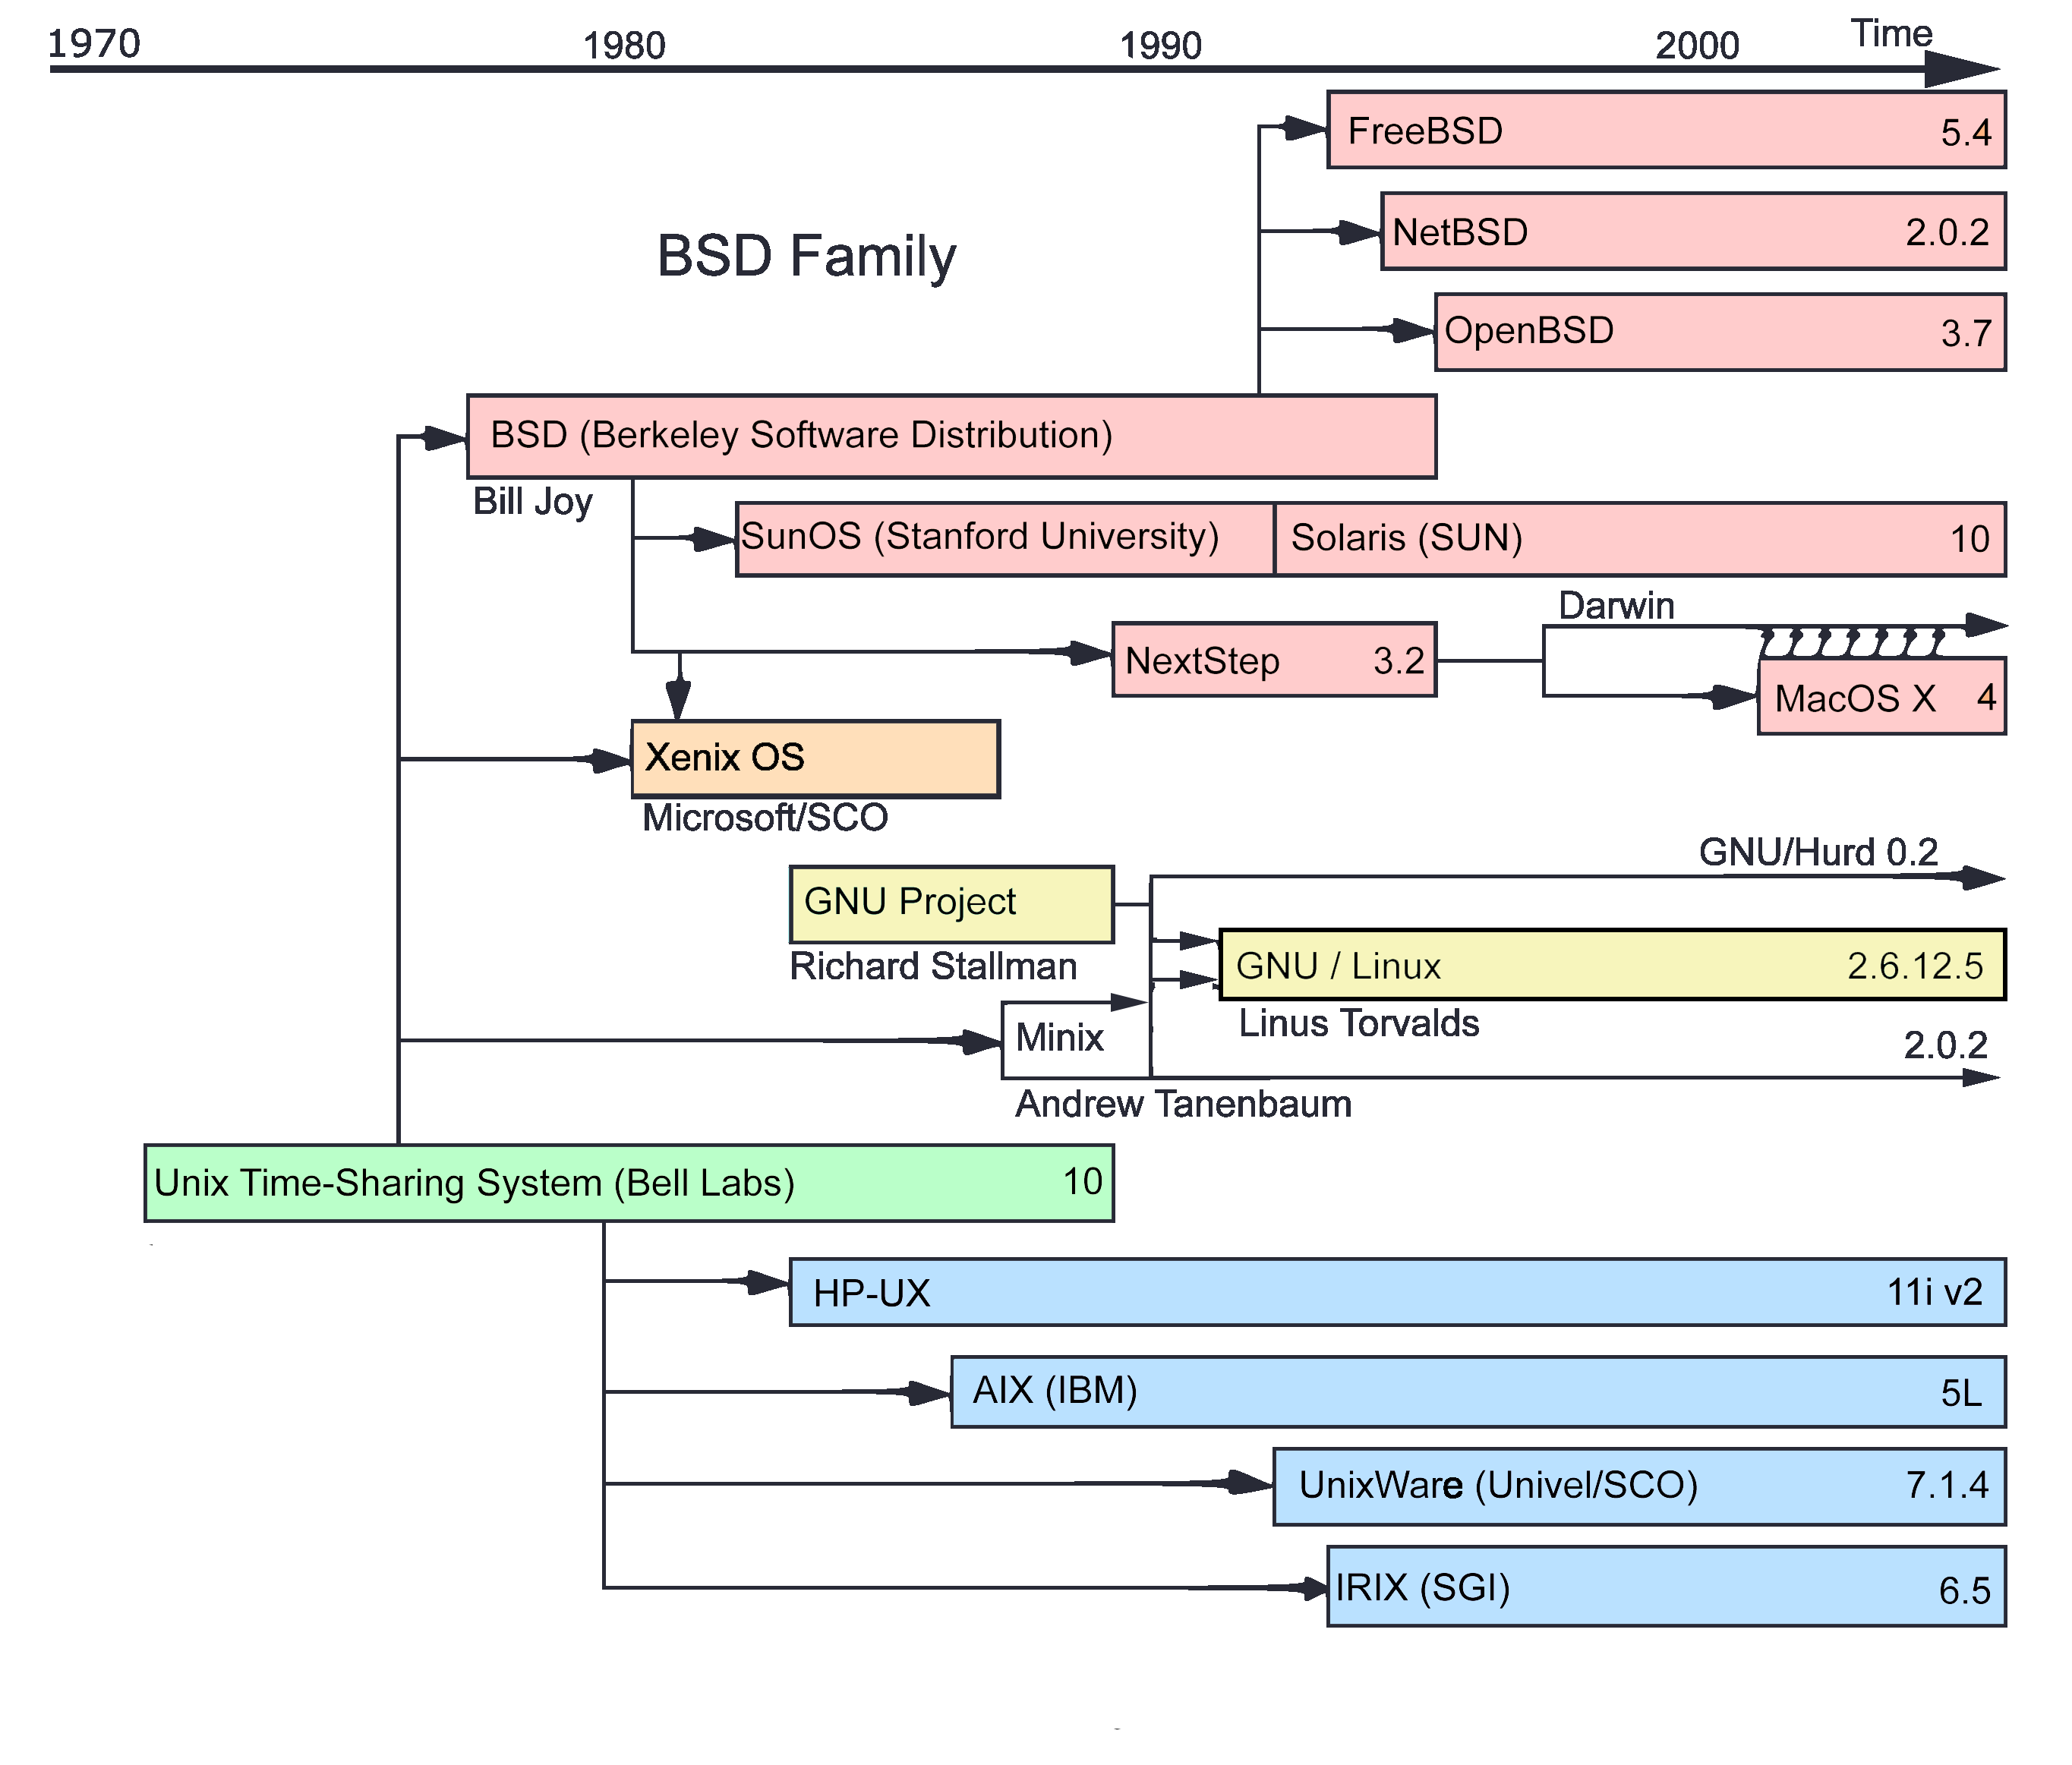
\includegraphics[width=1\textwidth]
    {Timeline_of_Unix_families}
    \caption{История развития UNIX-систем.}
    \label{fig:hist}
\end{figure}

\begin{figure}[h]
    \centering
    
\includegraphics[width=220px]{UNIX.png}
    \caption{Логотип UNIX}
    \label{fig:UNIX_symbol}
\end{figure}

\begin{figure}[h]
    \centering
    
\includegraphics[width=125px]
    {128px-Heckert_GNU_white.png}
    \caption{Логотип GNU}
    \label{fig:GNU_symbol}
\end{figure}

\begin{figure}[t]
    \centering
    
\includegraphics[width=100px]{Tux.png}
    \caption{Талисман Linux - пингвин Tux}
    \label{fig:linux_symbol}
\end{figure}

\begin{figure}[t]
    \centering
    
\includegraphics[width=100px]{BVXyPwe.png}
    \caption{Логотип Minix}
    \label{fig:minix_symbol}
\end{figure}

\section{Семейства дистрибутивов Linux}

\begin{longtable}{|p{0.3\textwidth}|
p{0.7\textwidth}|}
    \hline
        Ориентация & Основные представители\\\hline
        Дистрибутивы общего назначения & 
        \begin{minipage}{\textwidth}
        \begin{list}{•}{~}
            \item Fedora Core
            \item Debian GNU/Linux
            \item SuSE
            \item Mandrakelinux
            \item Slackware
            \item ALT Linux
            \item ASP Linux
            \item Gentoo
            \item Linux From Scratch
            \item Linspire
            \item PLD Linux Distribution
            \item Red Flag Linux
            \item Sorcerer GNU/Linux
            \item Source Mage
            \item Turbolinux
            \item Ubuntu Linux
            \item Xandros
        \end{list}
        ~
        \end{minipage}
    \\\hline
    \smallskip Дистрибутивы для мэйнфреймов& 
    \begin{list}{•}{~} \item 
    Linux on zSeries\end{list}
    \\\hline
    Серверные дистрибутивы &
    \begin{minipage}{\textwidth}
        \begin{list}{•}{~}
            \item Red Hat Enterprise Linux
            \item SuSE Linux Enterprise Server
            \item SuSEALT Linux Master
            \item ASP Linux Server
            \item LTSP
        \end{list}
        ~
    \end{minipage}
    \\\hline
    Защищенные дистрибутивы &
    \begin{minipage}{\textwidth}
        \begin{list}{•}{~}
            \item Trustix
            \item SELinux
            \item Tinfoil Hat Linux
            \item Trinux
            \item "Утес-К"
        \end{list}
        ~
    \end{minipage}
    \\\hline
    Дистрибутивы для мультимедиа &
    \begin{minipage}{\textwidth}
        \begin{list}{•}{~}
            \item MoviX
            \item Agnula
            \item Dynebolic
        \end{list}
        ~
    \end{minipage}
    \\\hline
    Дистрибутивы для маршрутизаторов и файерволов &
    \begin{minipage}{\textwidth}
        \begin{list}{•}{~}
            \item Coyote Linux
            \item Linux Router Project
            \item Gibraltar
            \item IPCop Firewall
            \item Sentry Firewall
            \item SmoothWall
        \end{list}
        ~
    \end{minipage}
    \\\hline
    Дистрибутивы для встроенных систем &
    \begin{minipage}{\textwidth}
        \begin{list}{•}{~}
            \item Embedded Debian
            \item ELKS Linux
            \item Linux Microcontroller Project
        \end{list}
        ~
    \end{minipage}
    \\\hline
    Дистрибутивы для "слабых" компьютеров &
    \begin{minipage}{\textwidth}
        \begin{list}{•}{~}
            \item Vector Linux
            \item Vector Linux
            \item ttylinux
        \end{list}
        ~
    \end{minipage}
    \\\hline
    Дистрибутивы для USB &
    \begin{minipage}{\textwidth}
        \begin{list}{•}{~}
            \item Flonix
            \item Flash Puppy
            \item SPBLinux
        \end{list}
        ~
    \end{minipage}
    \\\hline
    Дистрибутивы, запускаемые из-под Windows &
    \begin{minipage}{\textwidth}
        \begin{list}{•}{~}
            \item Cooperative Linux
        \end{list}
        
    \end{minipage}
    \\
    \hline
\end{longtable}

\end{document}